\section{Task 1}
\subsection{Problem Statement}
Implement and compare Insertion Sort, Counting Sort, and Merge Sort based on
various input size on randomly generated data.  The comparison metric should be
the execution time of each sorting algorithm.
\subsection{Code}
\begin{code}
    \caption{Code for generating random numbers and saving into a file nums.txt}
    \cppcode{../random_number.cpp}
    \label{code:random}
\end{code}

\begin{code}
    \caption{Code for insertion sort}
    \cppcode{../insertion_sort.cpp}
    \label{code:insertion}
\end{code}

\begin{code}
    \caption{Code for merge sort}
    \cppcode{../merge_sort.cpp}
    \label{code:merge}
\end{code}

\begin{code}
    \caption{Code for counting sort}
    \cppcode{../counting_sort.cpp}
    \label{code:counting}
\end{code}

\begin{code}
    \caption{Makefile}
    \inputminted[fontsize=\small]{make}{../Makefile}
\end{code}

\subsection{Output}
\begin{figure}[H]
    \centering
    \begin{subfigure}[b]{0.4\textwidth}
        \centering
        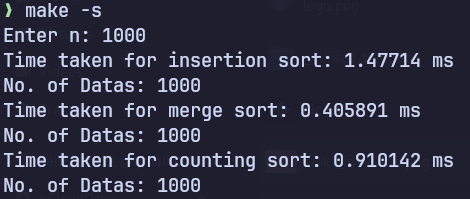
\includegraphics[width=\textwidth]{./img/out-1.png}
        \caption{Execution time for n=1000}
    \end{subfigure}
    \hfill
    \begin{subfigure}[b]{0.4\textwidth}
        \centering
        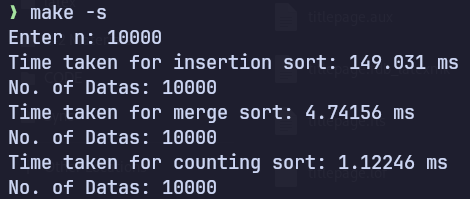
\includegraphics[width=\textwidth]{./img/out-2.png}
        \caption{Execution time for n=10000}
    \end{subfigure}
    \hfill
    \begin{subfigure}[b]{0.4\textwidth}
        \centering
        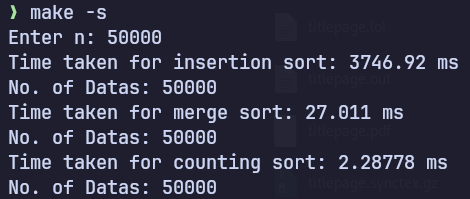
\includegraphics[width=\textwidth]{./img/out-3.png}
        \caption{Execution time for n=50000}
    \end{subfigure}
    \hfill
    \begin{subfigure}[b]{0.4\textwidth}
        \centering
        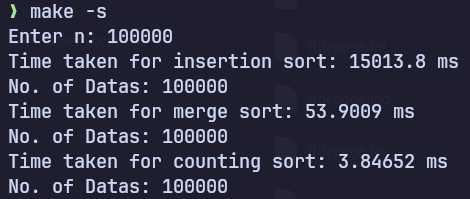
\includegraphics[width=\textwidth]{./img/out-4.png}
        \caption{Execution time for n=100000}
    \end{subfigure}
    
    \caption{Output for soting algorithm execution time}
    \label{fig:task1}

\end{figure}

\subsection{Result Analysis \& Discussion}
\begin{figure}[H]
    \centering
    \begin{subfigure}[b]{0.4\textwidth}
        \centering
        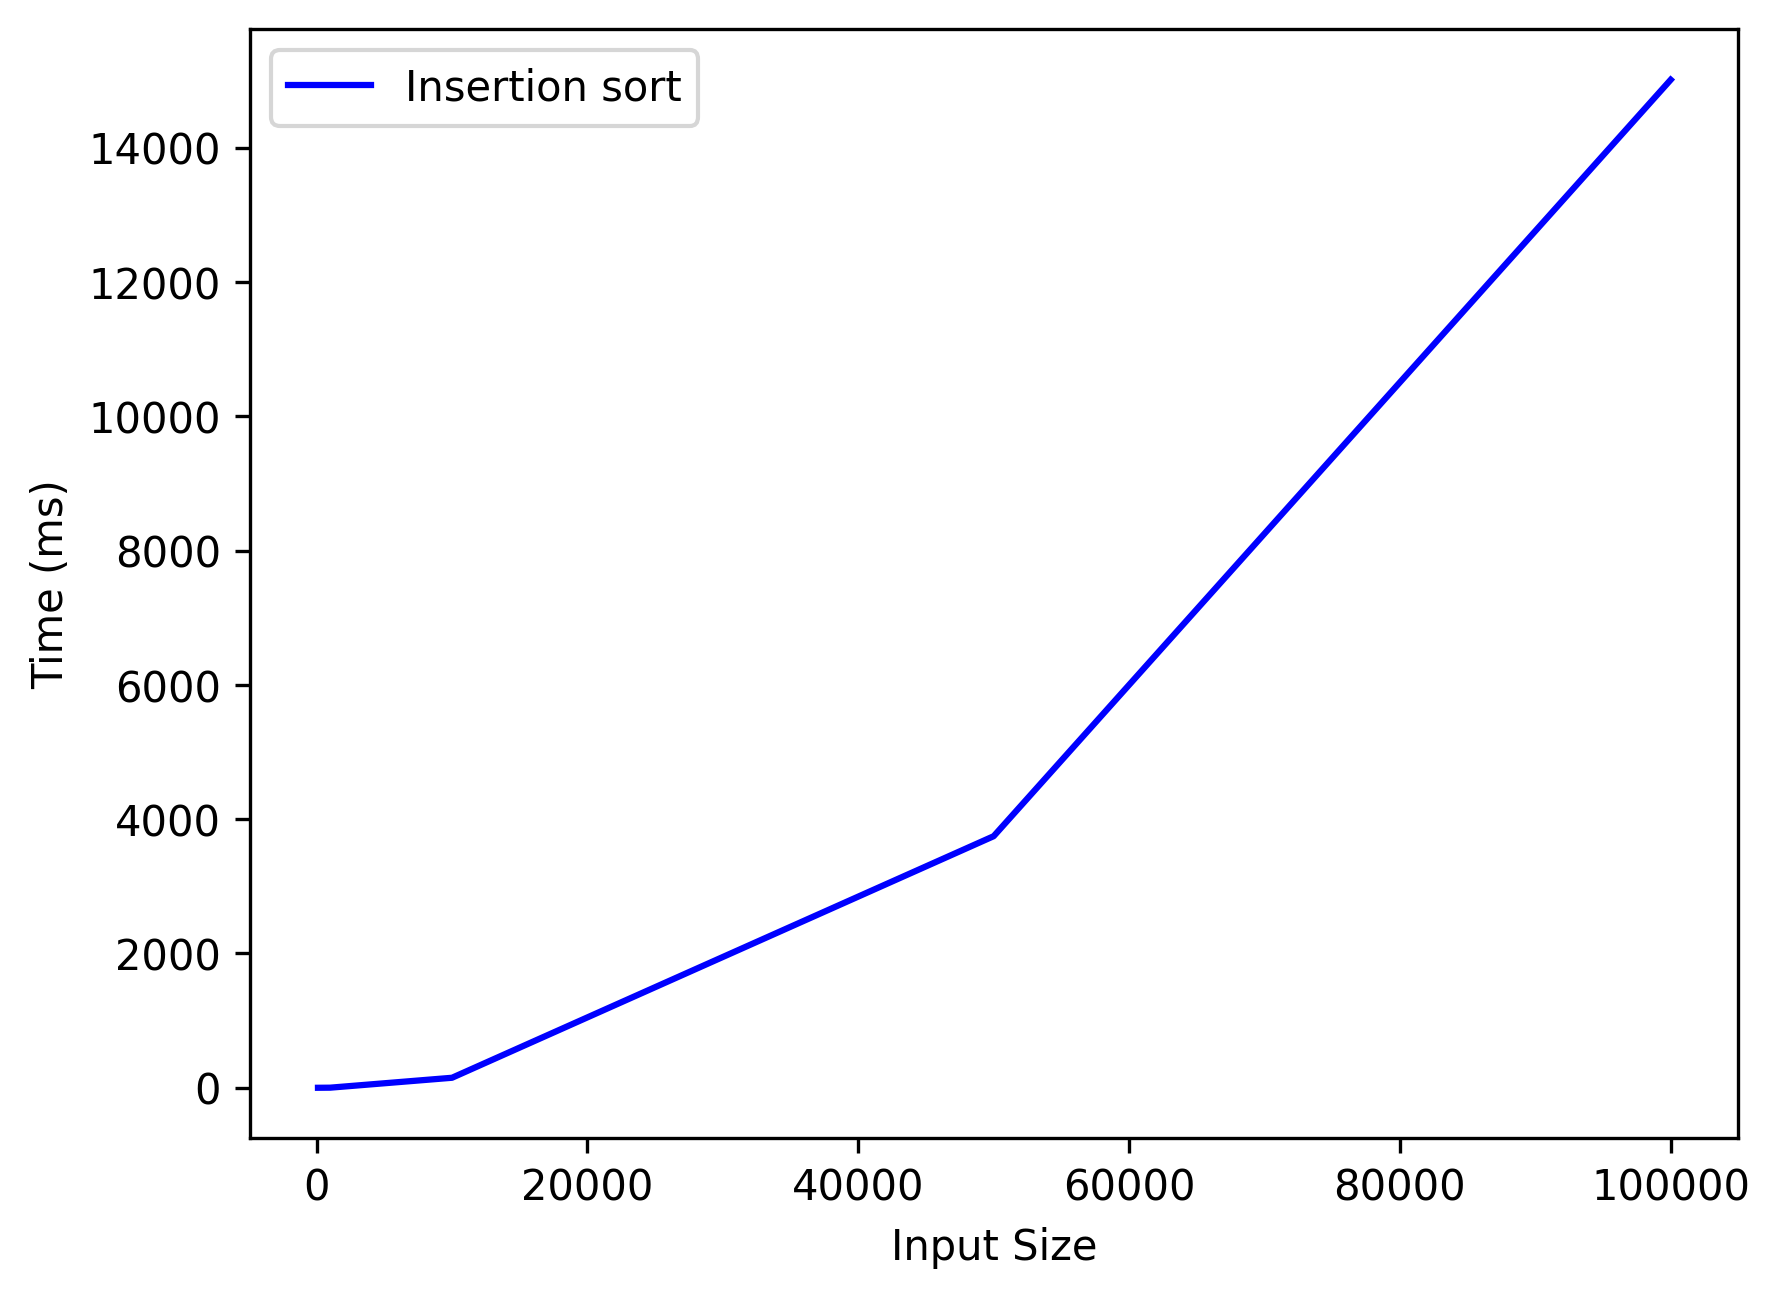
\includegraphics[width=\textwidth]{task1_insertion.png}
    \end{subfigure}
    \hfill
    \begin{subfigure}[b]{0.4\textwidth}
        \centering
        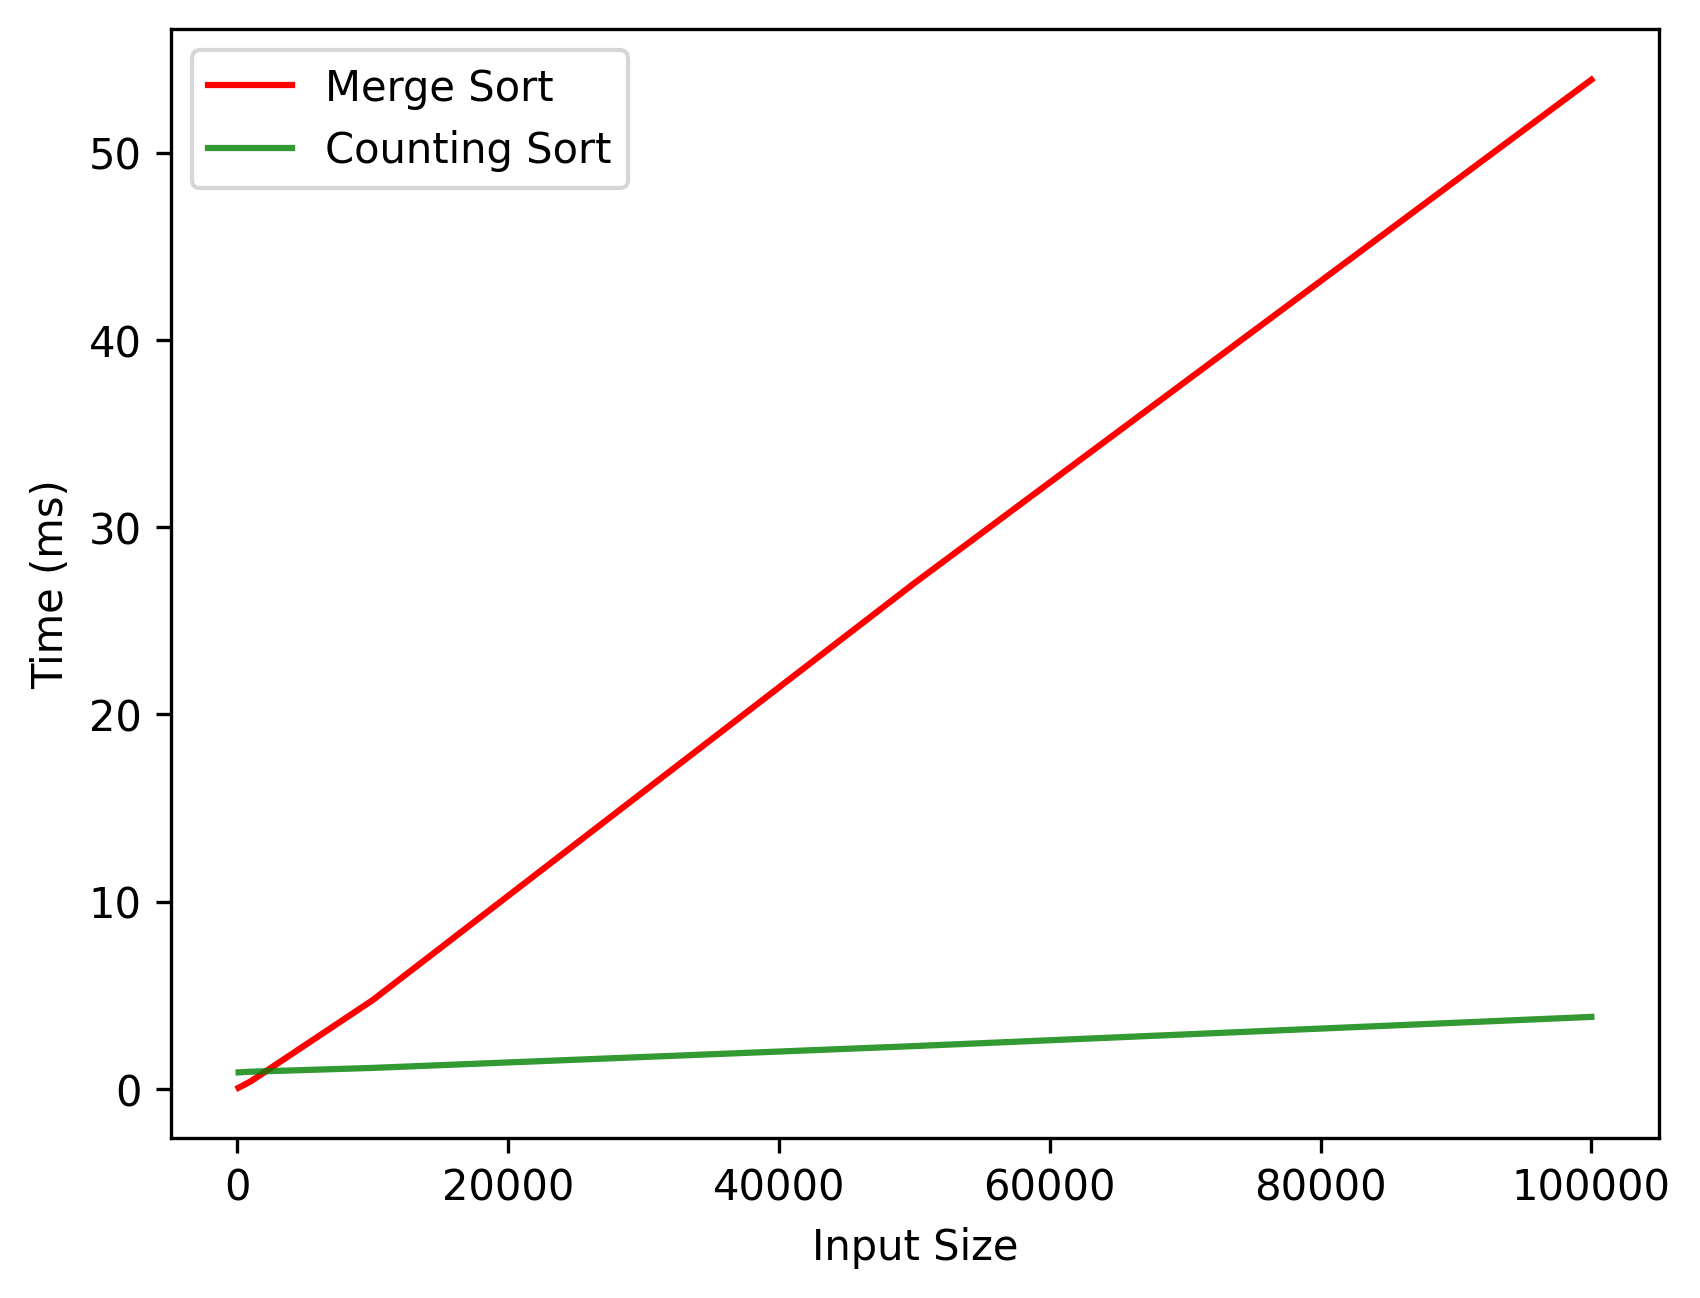
\includegraphics[width=\textwidth]{task1_merge_count.png}
    \end{subfigure}

    \caption{Time vs. Input size plot for insertion, merge and counting sort}
    \label{fig:task1plot}
\end{figure}

From \cref{fig:task1} we can see that as n approaches a large number
the execution time of
insertion sort is increasing in a fast manner.
By plotting the times in time vs input size
graph, see \cref{fig:task1plot} we can say that the time for insertion sort is 
increasing in a quadratic manner whereas for merge sort and counting sort 
time increases in a linear manner. But in case of merge sort the graph is not 
fully linear and more steeper than the counting sort. 
This property is similar to our known characteristics for insertion sort, merge sort and counting sort accordingly.
But counting sort have some limitations like random data range, and
unstable sorting if cummulative sum is not used. To implement the counting sort
we need to be cautious of these issues.
\newpage
\section{Task 2}
\subsection{Problem Statement}
Implement a Hybrid Sort algorithm where the algorithm switches from Merge Sort
to Insertion Sort when the size of the subarray to be conquered becomes smaller
than a threshold. Determine the optimal threshold empirically. Compare this
Hybrid Sort algorithm with Merge Sort  based on various input size and various
threshold on randomly generated data.
\subsection{Code}
\begin{code}
    \label{code:hybrid}
    \caption{Code for hybrid sort}
    \cppcode{../hybrid_sort.cpp}
\end{code}
\subsection{Output}

\begin{figure}[H]
    \centering
    \begin{subfigure}[t]{0.4\textwidth}
        \centering
        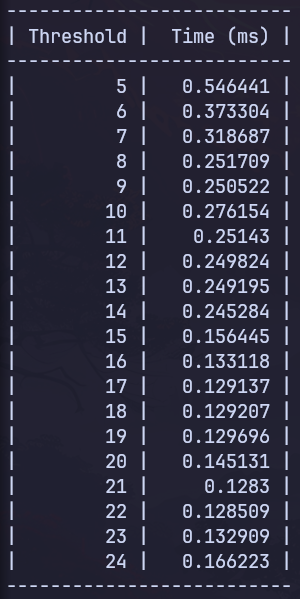
\includegraphics[scale=0.4]{img/task4/hi-1000.png}
        \caption{Hybrid sort for input size 1,000}
    \end{subfigure}
    \hfill
    \begin{subfigure}[t]{0.4\textwidth}
        \centering
        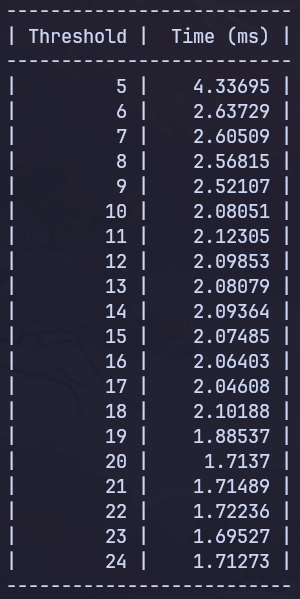
\includegraphics[scale=0.4]{img/task4/hi-10000.png}
        \caption{Hybrid sort for input size 10,000}
    \end{subfigure}
    \hfill
    \begin{subfigure}[t]{0.4\textwidth}
        \centering
        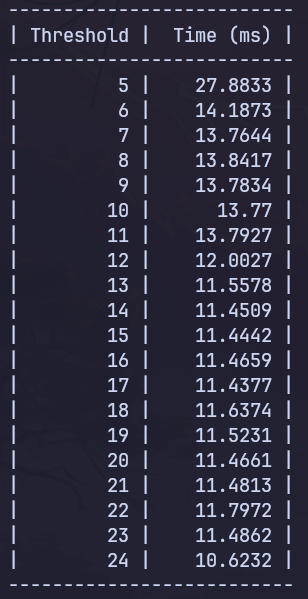
\includegraphics[scale=0.4]{img/task4/hi-50k.png}
        \caption{Hybrid sort for input size 50,000}
    \end{subfigure}
    \hfill
    \begin{subfigure}[t]{0.4\textwidth}
        \centering
        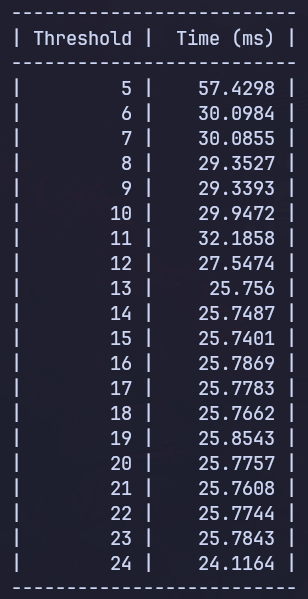
\includegraphics[scale=0.4]{img/task4/hi-1lac.png}
        \caption{Hybrid sort for input size 1,00,000}
    \end{subfigure}
    \caption{Hybrid sort execution time for various threshold values \&
    various input size}
    \label{fig:task2}
\end{figure}

\subsection{Result Analysis \& Discussion}
\begin{figure}[H]
    \centering
    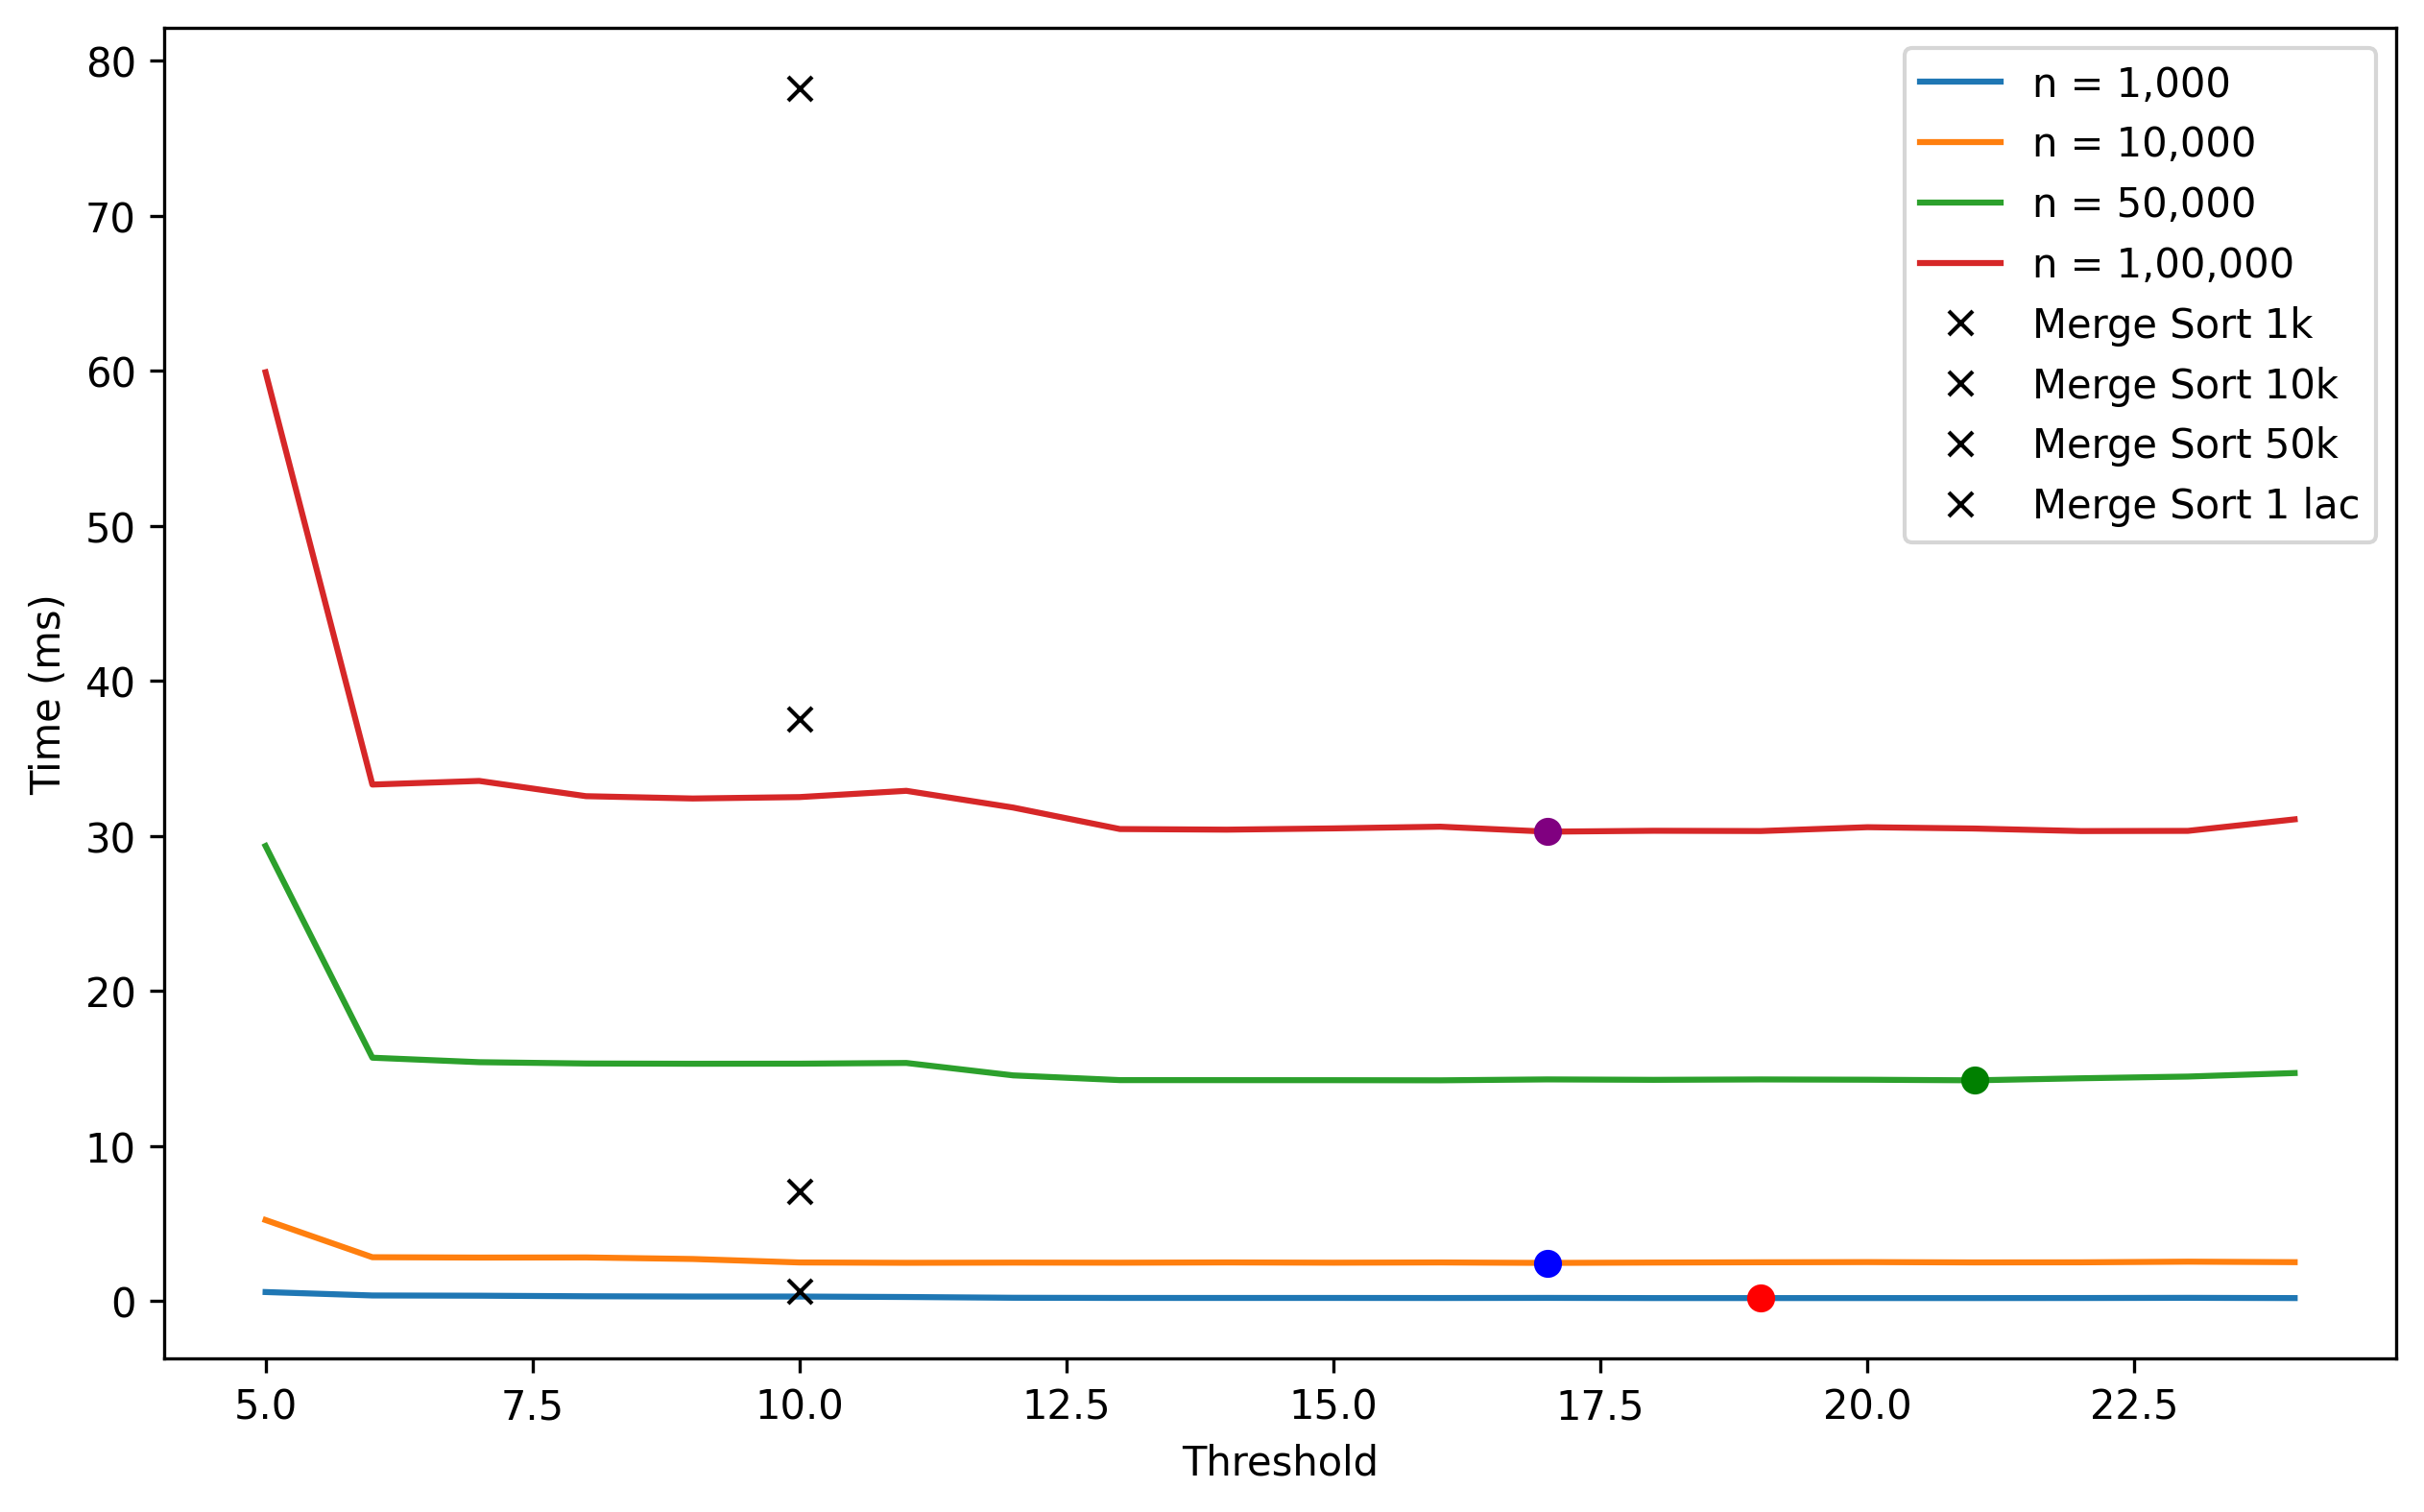
\includegraphics[width=\textwidth]{img/task2/task2_performance_comparison.png}
    \caption{Performance comparison of hybrid sort across various data sizes for various thresholds}
    \label{fig:task2plot}
\end{figure}
From \cref{fig:task2plot} it can be easily said that with increasing input size \textit{n} the threshold value for hybrid sort using insertion sort also increases.
For input size 1,000 we obtain a threshold around 21, for n = 10,000 threshold becomes approximately 23 and for the last two the value is 25.
% And this is the expected characteristics, because when the input size is
% increasing, the complexity for insertion sort is also increasing

In case of merge sort (see \cref{code:merge}), we know that merge sort doesn't depend on any thresholds,
rather in every case it follows an avarage case complexity of 
$\mathbb{O}(n\log n)$
\newpage
\section{Task 3}
\subsection{Problem Statement}
Take the Hybrid Sort algorithm from Task 2, instead of Insertion Sort, use
Bubble Sort. Determine the optimal threshold empirically. Make a 3-way
comparison between Merge Sort, Hybrid Sort with Insertion Sort, Hybrid Sort
with Bubble Sort algorithm based on various input size and various threshold on
randomly generated data.
\subsection{Code}
\begin{code}
    \label{code:bubble}
    \caption{Code for hybrid sort with bubble sort}
    \cppcode{../bubble.cpp}
\end{code}

\subsection{Output}
For hybrid sort with insertion sort, see \cref{fig:task2}

\textbf{Output for hybrid sort with bubble sort:}
\begin{figure}[H]
    \centering
    \begin{subfigure}[t]{0.4\textwidth}
        \centering
        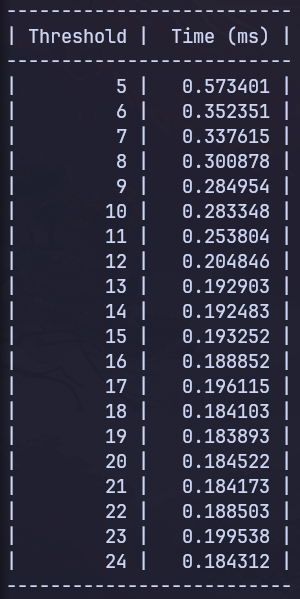
\includegraphics[scale=0.4]{img/task4/hb-1000.png}
        \caption{Hybrid sort for input size 1,000}
    \end{subfigure}
    \hfill
    \begin{subfigure}[t]{0.4\textwidth}
        \centering
        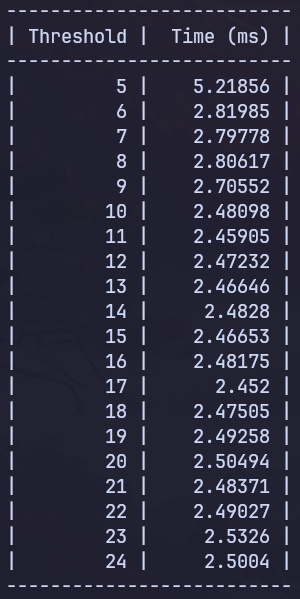
\includegraphics[scale=0.4]{img/task4/hb-10000.png}
        \caption{Hybrid sort for input size 10,000}
    \end{subfigure}
    \hfill
    \begin{subfigure}[t]{0.4\textwidth}
        \centering
        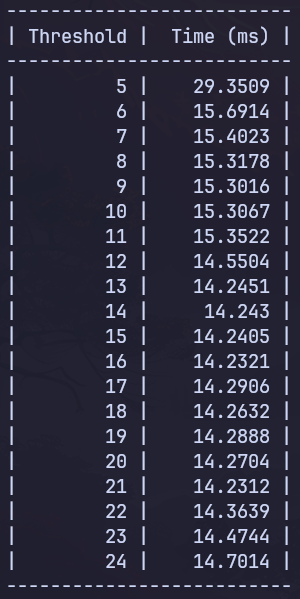
\includegraphics[scale=0.4]{img/task4/hb-50k.png}
        \caption{Hybrid sort for input size 50,000}
    \end{subfigure}
    \hfill
    \begin{subfigure}[t]{0.4\textwidth}
        \centering
        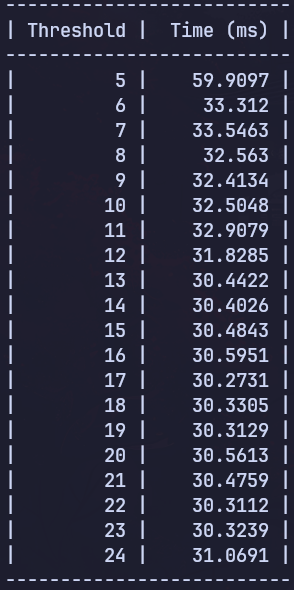
\includegraphics[scale=0.4]{img/task4/hb-1lac.png}
        \caption{Hybrid sort for input size 1,00,000}
    \end{subfigure}
    \caption{Hybrid sort with bubble sort execution time for various threshold values \&
    various input size}
    \label{fig:task3}
\end{figure}
\subsection{Result Analysis \& Discussion}
\begin{figure}[H]
    \begin{center}
        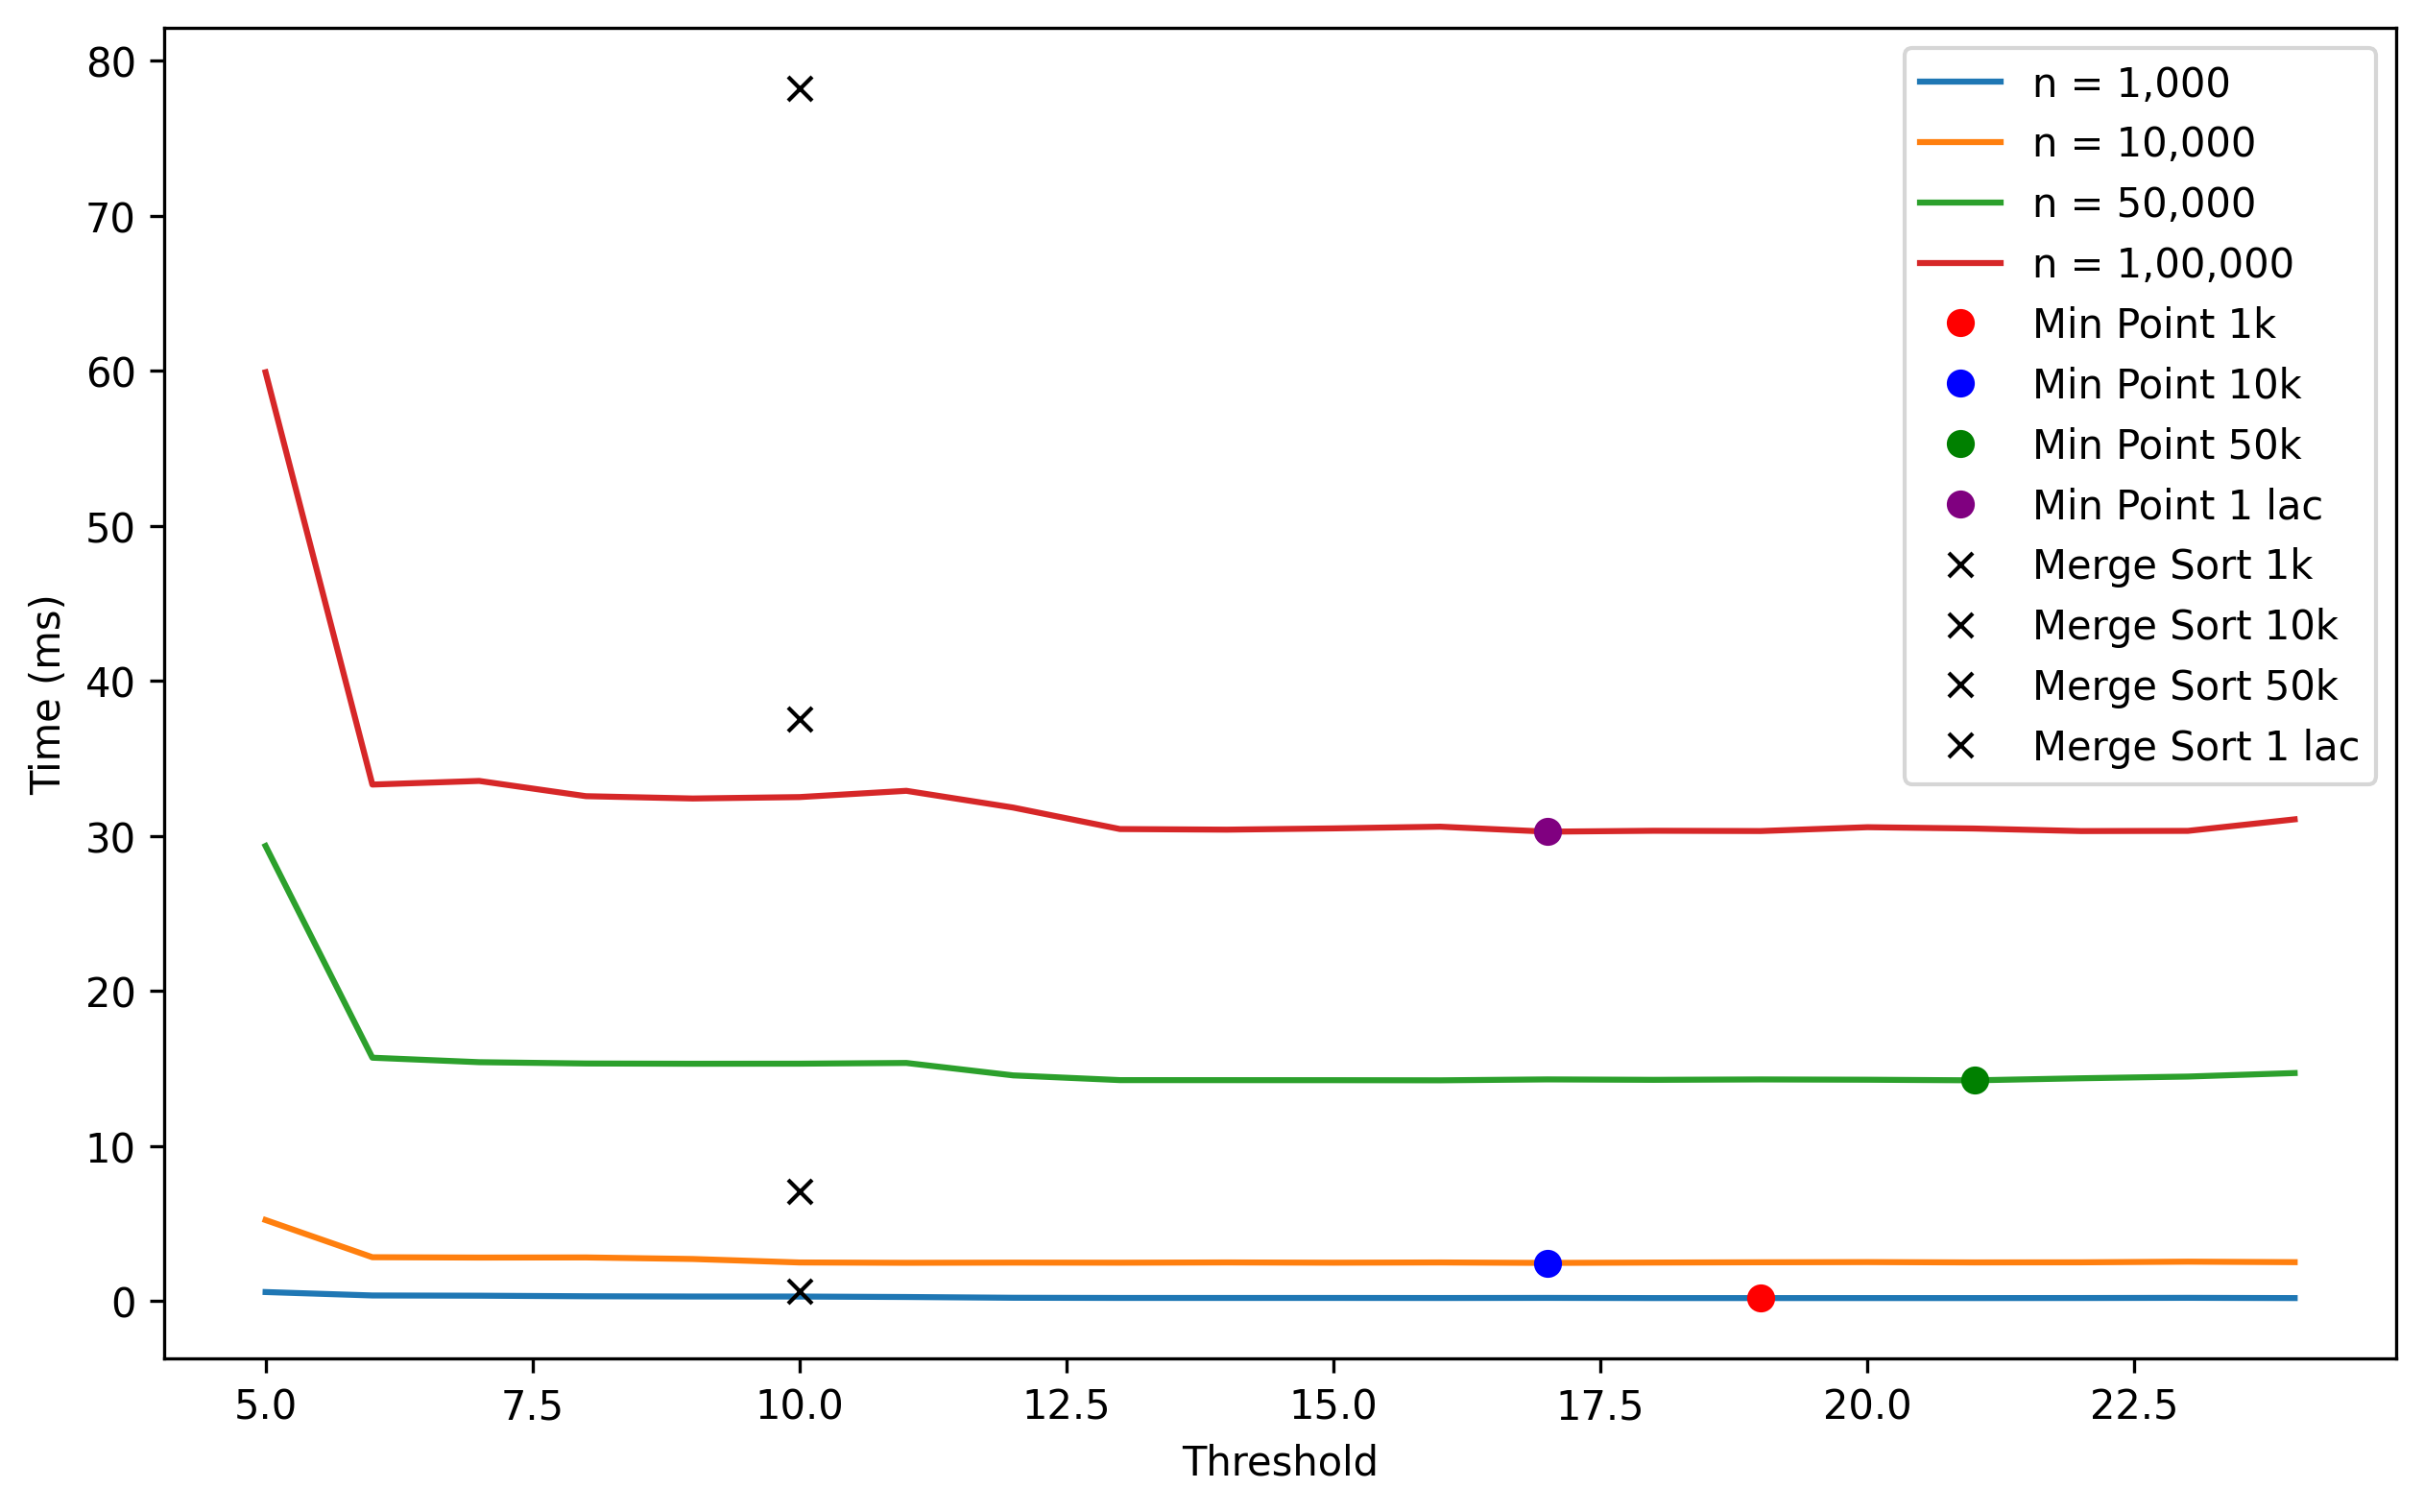
\includegraphics[width=\textwidth]{img/task3_performance_comparison_bubble.png}
    \end{center}
    \caption{Performance comparison of hybrid sort using bubble sort across various data sizes for various thresholds}
    \label{fig:task3plot}
\end{figure}


\begin{table}[H]
    \centering
    \caption{3-way comparison table for merge \& hybrid sort}
    \label{tab:comp}
\begin{tabular}{lrrr}
    \toprule
    \multicolumn{4}{c}{Execution time (ms)} \\
    \cmidrule(r){2-4}
    Input Size & Merge Sort & Hybrid w/ insertion sort & Hybrid w/ bubble sort \\
    \midrule
    1000 & 0.625851 & 0.1283, th 21 & 0.183893, th 19\\
    10,000 & 7.05903 &  1.69527, th 23 &  2.452, th 17\\
    50,000 & 37.5342 & 10.6232, th 24 &14.2312, th 21\\
    1,00,000 & 78.2175  & 24.1164, th 24& 30.2731, th 17 \\
    \bottomrule
\end{tabular}
\end{table}

From \cref{fig:task2plot}, \cref{fig:task3plot} it can be said that hybrid
sort significantly reduces the execution time than merge sort. And with
appropriate threshold value both of the hybrid sort outperforms merge
sort, which is shown in \cref{tab:comp}.

In conclusion, the implementation is consistent with the expected outcome,
because for small data size insertion sort and bubble sort performs better than
merge sort. By taking the advantage of this property, both hybrid sort using
insertion sort and hybrid sort using bubble sort was implemented so that for 
a certain threshold value the merge sort will not be used. And this increases 
the execution time significantly.

\newpage
\section{Task 4}
\subsection{Problem Statement}
HackerLand National Bank has a simple policy for warning clients about possible fraudulent account activity. If the amount spent by a client on a particular day is greater than or equal to  the client's median spending for a trailing number of days, they send the client a notification about potential fraud. The bank doesn't send the client any notifications until they have at least that trailing number of prior days' transaction data.

Given the number of trailing days  and a client's total daily expenditures for a period of  days, determine the number of times the client will receive a notification over all  days.

\textbf{Input Format}

The first line contains two space-separated integers  and , the number of days of transaction data, and the number of trailing days' data used to calculate median spending respectively.
The second line contains  space-separated non-negative integers where each integer  denotes .

\textbf{Constraints}
\begin{itemize}
    \item $ 1 \le n \le 2\times10^5  $
    \item $ 1\le d \le n $
    \item $ 0 \le expenditure[i] \le 200 $ 
\end{itemize}

\subsection{Code}
\begin{code}
    \label{code:fradulent}
    \caption{Code for Fradulent Activity Notifications}
    \cppcode{../fradulent.cpp}
\end{code}

\subsection{Output}
\begin{figure}[H]
    \begin{center}
        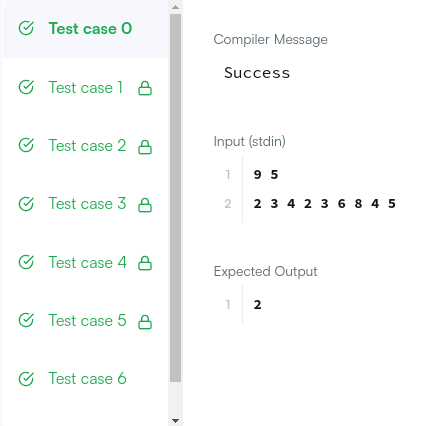
\includegraphics[scale=0.5]{img/fradulent_ac.png}
    \end{center}
    \caption{Accepted screenshot for the problem}\label{fig:}
\end{figure}

